
\section{The prop \texorpdfstring{$\M$}{M}} \label{s:operads and props}

We now review the definition of the finitely presented prop $\M$ introduced in \cite{medina2020prop1} and whose associated operad is a model for the  $E_\infty$-operad.
Given its small number of generators and relations, is well suited to define $E_\infty$-structures.
In the next section we use this model to define natural $E_\infty$-structures on cubical chains and cochains.
We start by reviewing the basic material in the theory of operads and props, referring the reader to, for example, \cite{markl2008props} for a more complete treatment.

\subsection{Symmetric modules and bimodules}

Let $\S$ be the category whose objects are the natural numbers and whose set of morphisms between $m$ and $n$ is empty if $m \neq n$ and is otherwise the symmetric group $\S_n$.
A \textit{left $\S$-module} (resp. \textit{right} $\S$-\textit{module} or $\S$-\textit{bimodule}) is a functor from $\S$ (resp. $\S^\op$ or $\S \times \S^\op$) to $\Ch$.
In this paper we prioritize left module structures over their right counterparts.
As usual, taking inverses makes both perspectives equivalent.
We respectively denote by $\smod$ and $\sbimod$ the categories of left $\S$-modules and of $\S$-bimodules with morphisms given by natural transformations.

The group homomorphisms $\S_n \to \S_n \times \S_1$ induce a forgetful functor
\[
\forget \colon \sbimod \to \smod,
\]
given explicitly by $\forget(\P)(r) = \P(1, r)$ for $r \in \N$.
The similarly defined forgetful functor to right $\S$-modules will not be used.

\subsection{Composition structures}

We can define \textit{operads} and \textit{props} by enriching $\S$-modules and $\S$-bimodules with certain composition structures.
For a complete presentation of these concepts we refer to Definition~11 and 54 of \cite{markl2008props}.
Intuitively, using examples defined in the next subsection, operads and props can be understood by abstracting the composition structure naturally present in the left $\S$-module $\End^C$ (or right $\S$-module $\End_C$), naturally an operad, and the $\S$-bimodule $\End^C_C$, naturally a prop.
We remark that the prop structure on $\P$ restricts to an operad structure on $\forget(\P)$.

\subsection{Representations}

Given a chain complex $C$ define
\begin{gather*}
\End^C(r) = \Hom(C, C^{\otimes r}), \qquad
\End_C(r) = \Hom(C^{\otimes r}, C), \\
\End^C_C(r, s) = \Hom(C^{\otimes r}, C^{\otimes s}),
\end{gather*}
with their natural operad and prop structures respectively.
We remark that the forgetful functor $\forget$ sends $\End^C_C$ to $\End^C$.

Let $C$ be a chain complex, $\O$ an operad, and $\P$ a prop.
An $\O$-\textit{coalgebra} (resp. $\O$-\textit{algebra} or $\P$-\textit{bialgebra}) structure on $C$ is a structure preserving morphism $\O \to \End^C$ (resp. $\O \to \End_C$ or $\P \to \End_C^C$).

\subsection{\pdfEinfty-operads}

Recall that a \textit{free $\S_r$-resolution} of a chain complex $C$ is a quasi-isomorphism $R \to C$ from a chain complex of free $\k[\S_r]$-modules.

An $\S$-module $M$ is said to be $E_{\infty}$ if there exists a morphism of $\S$-modules $M \to \underline{\k}$ inducing for each $r \in \N$ a free $\S_r$-resolution $M(r) \to \k$.

An operad is said to be $E_{\infty}$ if its underlying $\S$-module is $E_\infty$.

\subsection{Free prop construction} \label{ss:free prop}

\begin{figure}
	\boxed{\begin{tikzpicture}[scale=.6]
\draw (1,3.7) to (1,3); 

\draw (1,3) to [out=205, in=90] (0,0);

\draw [shorten >= 0cm] (.6,2.73) to [out=-100, in=90] (2,0);

\draw [shorten >= .15cm] (1,3) to [out=-25, in=30, distance=1.1cm] (1,1.5);
\draw [shorten <= .1cm] (1,1.5) to [out=210, in=20] (0,1);

\node at (1,3.9){};
\node at (0,-.32){};
\node at (2,-.32){};

\node at (3,1.5){$\sim$\ \ \ };
\end{tikzpicture}
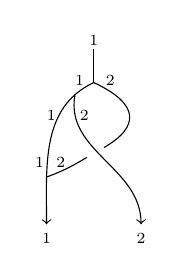
\begin{tikzpicture}[scale=.6]
\draw (1,3.7) to (1,3); 

\draw [->](1,3) to [out=205, in=90] (0,0);

\draw [shorten >= 0cm,->] (.6,2.73) to [out=-100, in=90] (2,0);

\draw [shorten >= .15cm] (1,3) to [out=-25, in=30, distance=1.1cm] (1,1.5);
\draw [shorten <= .1cm] (1,1.5) to [out=210, in=20] (0,1);


\def\x{.8}

\node[scale=\x] at (1,3.9){$\scriptstyle 1$};

\node[scale=\x] at (.7,3.05){$\scriptstyle 1$};
\node[scale=\x] at (1.35,3.05){$\scriptstyle 2$};

\node[scale=\x] at (.1,2.3){$\scriptstyle 1$};
\node[scale=\x] at (.8,2.3){$\scriptstyle 2$};

\node[scale=\x] at (-.15,1.3){$\scriptstyle 1$};
\node[scale=\x] at (.3,1.3){$\scriptstyle 2$};

\node[scale=\x] at (0,-.3){$\scriptstyle 1$};
\node[scale=\x] at (2,-.3){$\scriptstyle 2$};
\end{tikzpicture}}
	\caption{Immersed graphs represent labeled directed graphs with the direction implicitly given from top to bottom and the labeling from left to right.}
	\label{f:immersion}
\end{figure}

The \textit{free prop} $\free(M)$ generated by an $\S$-bimodule $M$ is constructed using isomorphism classes of directed graphs with no directed loops that are enriched with the following labeling structure.
We think of each directed edge as built from two compatibly directed half-edges.
For each vertex $v$ of a directed graph $\Gamma$, we have the sets $in(v)$ and $out(v)$ of half-edges that are respectively incoming to and outgoing from $v$.
Half-edges that do not belong to $in(v)$ or $out(v)$ for any $v$ are divided into the disjoint sets $in(\Gamma)$ and $out(\Gamma)$ of incoming and outgoing external half-edges.
For any positive integer $n$ let $\overline{n} = \{1, \dots, n\}$ and set $\overline{0} = \emptyset$.
For any finite set $S$, denote the cardinality of $S$ by $|S|$.
The labeling is given by bijections
\[
\overline{|in(\Gamma)|}\to in(\Gamma), \qquad
\overline{|out(\Gamma)|}\to out(\Gamma),
\]
and
\[
\overline{|in(v)|}\to in(v), \qquad
\overline{|out(v)|}\to out(v),
\]
for every vertex $v$.
We refer to the isomorphism classes of such labeled directed graphs with no directed loops as $(n,m)$\textit{-graphs} denoting the set of these by $\graphs(m,n)$.
We use graphs immersed in the plane to represent elements in $\graphs(m,n)$, please see \cref{f:immersion}.
We consider the right action of $\S_n$ and the left action of $\S_m$ on a $(n,m)$-graph given respectively by permuting the labels of $in(\Gamma)$ and $out(\Gamma)$.
This action defines the $\S$-bimodule structure on the free prop
\begin{equation} \label{e:free prop}
\free(M)(m,n) \ = \bigoplus_{\Gamma \in \graphs(m,n)} \bigotimes_{v \in Vert(\Gamma)} out(v) \otimes_{\S_q} M(p, q) \otimes_{\S_p} in(v),
\end{equation}
where we simplified the notation writing $p$ and $q$ for $\overline{|in(v)|}$ and $\overline{|out(v)|}$ respectively.
The composition structure is defined by (relabeled) grafting and disjoint union.

\subsection{The prop $\M$}

We now recall the model of $E_\infty$ that is central to our constructions.

\begin{definition}
	Let $\M$ be the prop generated by
	\begin{equation} \label{e:generators of M}
	\counit\,, \hspace*{.6cm} \coproduct\,, \hspace*{.6cm} \product,
	\end{equation}
	in degrees $0$, $0$ and $1$ respectively, and boundaries
	\begin{equation} \label{e:boundary of M}
	\partial\ \counit = 0,
	\hspace*{.6cm}
	\partial\, \coproduct = 0,
	\hspace*{.6cm}
	\partial \product = \ \boundary\,,
	\end{equation}
	modulo the prop ideal generated by
	\begin{equation} \label{e:relations of M}
	\leftcounitality\,, \hspace*{.6cm} \rightcounitality\,, \hspace*{.6cm} \productcounit.
	\end{equation}
\end{definition}

Explicitly, any element in $\M(m,n)$ can be written as a linear combination of the $(m,n)$-graphs generated by those in \eqref{e:generators of M} via grafting, disjoint union and relabeling, modulo the prop ideal generated by the relations in \eqref{e:relations of M}. Its boundary is determined, using \eqref{e:free prop}, by \eqref{e:boundary of M}.

As proven in \cite[Theorem 3.3]{medina2020prop1} we have the following.

\begin{proposition}
	The operad $\UM$ is $E_{\infty}$.
\end{proposition}

We remark that, as proven in \cite{medina2018prop2}, this prop is obtained from applying the functor of cellular chains to a finitely presented prop over the category of CW-complexes.

\subsection{Hopf operads and $E_\infty$-bialgebras}

So far we have consider operad and props over the category $\Ch$ but, since $\coAlg$ is also a symmetric monoidal category, we can consider them over $\coAlg$.
That is to say, demand that all defining chain complexes be coalgebras and all compositions be morphisms of these.
We refer to operads and props over $\coAlg$ as \textit{Hopf operads and props} respectively.

If $\O$ is a Hopf operad, the category $\coAlg_\O$ is monoidal.
The structure maps of a product of $\O$-coalgebras $C \otimes C^\prime$ are given by
\[
\begin{tikzcd} [column sep = normal, row sep=normal]
\O(r) \otimes (C \otimes C^\prime) \arrow[r, "\Delta_\O \otimes \id"] &[10 pt]
\O(r) \otimes \O(r) \otimes (C \otimes C^\prime) \arrow[d, "Sh"'] & \\ &
\big(\O(r) \otimes C \big) \otimes \big( \O(r) \otimes C \big) \arrow[r] &
C^{\otimes r} \otimes C^{\prime\, \otimes r} \arrow[d, "Sh"] & \\ & &
(C \otimes C^\prime)^{\otimes r}.
\end{tikzcd}
\]
Similarly, if $\P$ is a Hopf prop then its category of representations is also monoidal.

\subsection{Hopf structure on $\M$} \label{ss:hopf prop M}

As proven in \cite{medina2021cobar}, the prop $\M$ is Hopf with coproduct $\Delta_\M$ and counit $\varepsilon_\M$ induced by
\begin{align*}
\coproduct & \mapsto \coproduct \otimes \coproduct \,, &
\coproduct & \mapsto 1, \\
\counit \ & \mapsto \ \counit \ \otimes \ \counit \,, &
\counit \ & \mapsto 1, \\
\product & \mapsto \rightboundary \otimes \product + \product \otimes \leftboundary \,, &
\coproduct & \mapsto 0.
\end{align*}
It follows from the previous subsection that $\coAlg_\UM$ is a monoidal category.

\subsection{Simplicial $E_{\infty}$-structure} \label{ss:e-infty on simplicial}

We review from \cite{medina2020prop1} a natural $\mathcal M$-structure on the chains of standard simplices.
These define, for any simplicial set, a natural $\UM$-structure on its chains generalizing the $E_{\infty}$-coalgebra structures constructed by McClure--Smith \cite{mcclure2003multivariable} and Berger--Fresse \cite{berger2004combinatorial}.

An $\M$-structure is specified by three linear maps, the images of the generators
\[
\counit, \quad \coproduct, \quad \product,
\]
satisfying the relations in the presentation of $\mathcal M$.
For the chains on standard simplices, the first two generators are send respectively to the counit and coproduct of the Alexander--Whitney coalgebra as defined in \cref{ss:aw coalgebra}, and the third generator to an algebraic version of the join $\ast \colon \chains(\simplex^n)^{\otimes 2} \to \chains(\simplex^n)$ defined by
\[
\left[v_0, \dots, v_p \right] \ast \left[v_{p+1}, \dots, v_q\right] = \begin{cases} (-1)^{p+|\pi|} \left[ v_{\pi(0)}, \dots, v_{\pi(q)} \right] & \text{ if } v_i \neq v_j \text{ for } i \neq j, \\
0 & \text{ otherwise}, \end{cases}
\]
where $\pi$ is the permutation that orders the totally ordered set of vertices, and $(-1)^{|\pi|}$ its sign.

The same proof given in \cite[Theorem 4.2]{medina2020prop1} establishes the following.

\begin{proposition} \label{p:simplicial chain bialgebra}
	For every $n \in \mathbb{N}$, the assignment
	\[
	\counit \mapsto \epsilon, \quad \coproduct \mapsto \Delta, \quad \product \mapsto \ast,
	\]
	defines a natural $\mathcal M$-structure on $\chains(\simplex^n)$ extending the Alexander--Whitney coalgebra.
\end{proposition}

The chains on general simplicial sets are not equipped with an $\M$-structure, but using the forgetful functor from $\biAlg_{\M}$ to the cocomplete category $\coAlg_\UM$ allows us to Yoneda extend the induced natural $\UM$-structures on standard simplices to all simplicial sets.
Specifically, we obtain an extension of the Alexander--Whitney coalgebra in the form of a lift:
\[
\begin{tikzcd}[column sep=normal, row sep=small]
& \coAlg_\UM \arrow[d] \\
\sSet \arrow[r, "\schains"]
\arrow[ur, "\schainsUM", out=60, in=180]
& \Ch.
\end{tikzcd}
\]

\subsection{Multisimplicial \pdfEinfty-structure}

Since $\coAlg_\UM$ is monoidal we have a canonical functor $\coAlg_\UM^{\otimes k} \to \coAlg_\UM$ that we use to define a lift of the functor of multisimplicial chains to the category of $\UM$-coalgebras fitting in the following commutative diagram
\[
\begin{tikzcd}[column sep=huge, row sep=small]
& \coAlg_\UM^{\otimes k} \arrow[d] \\
& \coAlg_\UM \arrow[d] \\
\arrow[uur, "\schainsUM^{\otimes k}", out=90, in=180]
\arrow[ur, "\chains^{\msimplex{k}_\UM}", out=45, in=180, near end, dashed]
\sSet^k \arrow[r, "\schains"]
& \Ch.
\end{tikzcd}
\]

